\documentclass[conference]{IEEEtran}
\IEEEoverridecommandlockouts
% The preceding line is only needed to identify funding in the first footnote. If that is unneeded, please comment it out.
%Template version as of 6/27/2024

\usepackage{cite}
\usepackage{amsmath,amssymb,amsfonts}
\usepackage{graphicx}
\usepackage{float}
\usepackage{textcomp}
\usepackage{url}
\usepackage{huzaifa}
\usepackage{placeins}
\usepackage{adjustbox}
\usepackage{pifont}
\usepackage{array}
\usepackage{capt-of}
\def\BibTeX{{\rm B\kern-.05em{\sc i\kern-.025em b}\kern-.08em
    T\kern-.1667em\lower.7ex\hbox{E}\kern-.125emX}}
\begin{document}
\newcommand{\cmark}{\textcolor{green}{\ding{51}}}  % ✅ Define checkmark
\newcommand{\xmark}{\textcolor{red}{\ding{55}}}    % ❌ Define cross mark

% Cross
\[
\text{Cross symbol: } \times
\]

% Triangle
\[
\text{Triangle symbol: } \triangle
\]

% Circle
\[
\text{Circle symbol: } \circ
\]

% Square
\[
\text{Square symbol: } \square
\]





\title{Houdini: Security Benchmarking of Container Confinement}

\author{\IEEEauthorblockN{1\textsuperscript{st}}
\IEEEauthorblockA{\textit{Carleton University} \\
Ottawa, Canada \\
}
\and
\IEEEauthorblockN{2\textsuperscript{nd}}
\IEEEauthorblockA{\textit{Carleton University} \\
Ottawa, Canada \\
}
\and
\IEEEauthorblockN{3\textsuperscript{rd}}
\IEEEauthorblockA{\textit{Carleton University} \\
Ottawa, Canada \\
}
}

\maketitle

\begin{abstract}
  While container-based workloads are now a standard part of our cloud infrastructure, container security remains a challenging problem. Container confinement is a particularly pressing problem, as without it, a single vulnerable application can be used to compromise entire clusters of containers. While we have many technologies that can be used to secure containers, currently there is no easy way to determine whether a given Docker configuration provides even a basic level of protection. Here we present Houdini, a security test suite for container confinement. Much as network scanning tools can help catch misconfigured firewalls, Houdini can check whether a given Docker container configuration properly enforces confinement. While it can be used to test deployable containers, Houdini is optimised for testing and comparing container confinement technologies. Here we present the motivation, design, implementation, and initial results on running Houdini on a set of different container configurations. By providing a benchmark framework by which container confinement technologies can be evaluated, we believe Houdini can help foster the development of next-generation container confinement technologies.
\end{abstract}

\begin{IEEEkeywords}

\end{IEEEkeywords}

\section{Introduction}

Container-based workloads have become a cornerstone of modern cloud infrastructure, revolutionizing how applications are developed, deployed, and scaled, particularly within microservices architectures and DevOps workflows. Unlike hypervisor-based virtual machines (VMs), which each require a full operating system and rely on a hypervisor for hardware virtualization, containers are lightweight, share the host system’s kernel, and incur minimal overhead. This efficiency makes them exceptionally well-suited for continuous integration and rapid scaling, allowing organizations to optimize resource utilization and reduce costs while ensuring quick, consistent deployments. Furthermore, containers enable seamless portability by packaging all userspace dependencies into a unified image, thereby avoiding the common problem of environment-specific discrepancies. Yet, despite containers’ numerous benefits, they also introduce new security challenges, especially where container confinement is concerned.

Linux kernel features such as cgroups, namespaces, and mount points provide resource, process, and network isolation for containers. However, this separation is not foolproof. Kernel vulnerabilities, such as buffer overflows or privilege escalation flaws can allow a process to circumvent the very mechanisms designed to confine it. Misconfigurations can similarly open holes in container security, for instance by granting unnecessary capabilities, mounting sensitive host directories, or running containers in privileged mode. Finally, sophisticated attacks like container escapes exploit these weaknesses to break out of the container’s resource and namespace isolation. Once an attacker gains elevated privileges or direct access to the host system, they can disrupt other containers, exfiltrate data, or compromise the entire infrastructure. 

Technologies like SELinux, AppArmor, and seccomp provide additional layers of security to mitigate these issues, but are notoriously complex to configure and prone to misconfiguration. A best practices guide for container security~\cite{CIS} can help with configuring a container, but it offers no guarantee that the given configuration will perform as intended by the end-user. As container adoption has skyrocketed across industries, particularly in multi-tenant cloud environments, these security challenges have become more pronounced.

To address the discussed challenges, the cloud industry has developed technologies like gVisor\footnote{\url{https://gvisor.dev}} and Kata Containers\footnote{\url{https://katacontainers.io}}, which isolate containers further by running them within lightweight VMs. While this approach is effective, gVisor-based containers bypass seccomp confinement by intercepting and emulating syscalls instead of directly blocking them through seccomp, which could result in security vulnerabilities if the emulation logic is flawed. By developing methods to audit and validate confinement mechanisms, container security could be simplified by reducing reliance on such solutions.

Test suites play a crucial role in verifying that systems meet specified requirements and function correctly under defined conditions. They are widely used across computing disciplines, from performance benchmarking to security assessment. For instance, the Standard Performance Evaluation Corporation (SPEC) \cite{henning2000spec} is best known for developing industry-standard benchmarks that evaluate CPU performance and power efficiency, while the Transaction Processing Performance Council (TPC) \cite{10.1007/978-3-642-18206-8_1} establishes benchmarking standards for database performance. The Phoronix Test Suite \cite{zboril2025performance} is a widely used benchmarking tool, particularly for Linux-based systems, providing automated performance evaluations across various hardware and software configurations. 

%Beyond performance testing, test suites are essential in software development to prevent regressions. Many organizations mandate that all code changes pass a comprehensive suite of tests before integration. In production environments, test suites help maintain reliability through uptime monitoring, ensuring that services remain operational. 
Specialized security-focused test suites play a vital role in detecting vulnerabilities in deployed systems. Tools such as network scanners aid in identifying misconfigurations, outdated software versions, and unintended service exposures, helping organizations proactively mitigate security risks. However, a significant gap remains in the context of containers. There are currently no standardized or widely adopted test suites designed specifically to evaluate container confinement, functionality, or isolation effectiveness. This absence leaves organizations to rely on ad hoc methods, which are often inadequate for uncovering subtle misconfigurations or ensuring robust confinement. Given the growing reliance on containerized environments in modern infrastructure, the development of comprehensive test suites tailored for containers is imperative. Such test suites would not only address these critical gaps but also provide a reliable foundation for improving trust and security in containerized systems.

In this paper, we describe Houdini, the first test suite for verifying container confinement. Given a Docker container configuration (including the kernel, docker, and runc version), Houdini will instantiate the container in a standalone QEMU-based VM and perform multiple tests (or \textit{tricks}, as we call them) to evaluate whether the container is susceptible to various forms of misconfigurations or failures. These tests explore vulnerabilities that could disrupt container functionality, such as
%, but not limited to 
improper resource allocation, inadequate isolation, or insecure filesystem setups. Houdini is written in Python and is easily extensible, providing an extension language for writing controlled test cases 
%(which we refer to as "tricks") 
designed to evaluate whether a container confinement mechanism properly enforces security boundaries.

%In this paper, we describe the motivation, design, and implementation of Houdini. We also present the results of case studies by showing how Houdini can be used to detect misconfigured containers. 

%maybe better for the conclusion
%Our hope with Houdini is that it will help with the deployment of better confined containers and will support the development of new technologies to more reliably confine containers.

The rest of this paper proceeds as follows. Section~\ref{sec:container-confinment-problem} defines container confinement and associated challenges. Section~\ref{sec:motivation} further motivates the need for a container security test suite. We describe Houdini's design and implementation in Sections~\ref{sec:design} and~\ref{sec:implementation}. Section~\ref{sec:evaluation} presents three case studies demonstrating how Houdini can detect security issues, misconfigurations, and other inconsistencies. We review related work in Section~\ref{sec:related} and conclude in Section~\ref{sec:conclusion}.
\section{The Container Confinement Problem}
\label{sec:container-confinment-problem}


Container confinement can be defined as the set of mechanisms and strategies used to isolate a containerized application from the host system and other containers. Effective confinement is critical for maintaining system security and stability, as it ensures that containers operate within defined boundaries by restricting their access to system resources, processes, networks, inter-process communication (IPC), filesystems, devices, and kernel interfaces. 

A challenge with container confinement is that the level of confinement of a container is not fixed; it can vary based on the specific requirements or intentions of the user. In other words, the degree to which a container is isolated from the host system or other containers is customizable to meet the user’s needs. At one end of the spectrum, one can lock a container down so tightly that it is almost entirely isolated from the host system, which minimizes potential attack surfaces but can also render the container incapable of performing key tasks. On the other hand, allowing a container too much freedom undermines the security benefits of containerization by exposing more privileges than necessary. The optimal configuration, however, is one that strikes a balance between maximum confinement (restricting access to system resources as much as possible) and function flexibility (enabling the container to perform its intended tasks). Achieving this balance is the core problem and goal of container confinement.

A standard methodology for assessing container confinement is crucial due to the complexity of modern systems and the intricate vulnerabilities they present. A formal approach involving rigorously evaluating and analyzing the security of the container system might seem ideal, however, it is impractical because container environments are highly complex, with interactions between kernels, runtimes, orchestration tools, and external dependencies that are difficult to model comprehensively. Moreover, many vulnerabilities stem from subtle details that a formal model might overlook. Instead, an empirical approach offers a practical alternative. Though it will never be exhaustive, the goal is not comprehensive coverage but rather establishing a baseline set of tests that demonstrate effective container confinement. This approach is achievable and can evolve over time as new vulnerabilities are identified, allowing the methodology to remain current. Starting with tests for isolation, privilege escalation prevention, and resource limitation enforcement provides a solid foundation. By focusing on demonstrating security effectiveness in critical areas, this methodology can enhance confidence in container confinement while enabling continuous improvement and adaptation to the evolving threat landscape.
\section{Motivation}
\label{sec:motivation}

Houdini is designed to provide a systematic and reproducible approach to testing container confinement mechanisms. One of its primary goals is to evaluate whether container security features, such as namespaces, cgroups, seccomp, and Linux capabilities are effectively enforcing isolation. Many security tools rely on theoretical guarantees or static analysis, but Houdini focuses on empirical validation by executing controlled security tests that verify the correct enforcement of security mechanisms. By doing so, Houdini ensures that container security mechanisms are correctly configured.

Houdini is not only for testing container isolation but also as a means to optimize container configurations. By systematically simulating various tasks within different Docker containers, Houdini can help determine the minimal set of privileges required for a container to perform its intended function. For example, administrators can start with a container configured with broad privileges and then incrementally reduce permissions, such as Linux capabilities, seccomp filters, or resource limits, while monitoring task success. Houdini’s testing framework will identify the point at which functionality is maintained while unnecessary privileges are removed, thereby pinpointing the least privilege configuration that still allows the container to operate effectively. This approach is highly beneficial because it adheres to the principle of least privilege. Minimizing the privileges granted to a container reduces its attack surface, making it significantly harder for an attacker to exploit vulnerabilities.

Although runtime monitoring and anomaly detection, such as with eBPF-based tracing can provide immediate insights into container behavior, our goal isn't to implement an exhaustive, continuous surveillance system. Instead, we aim to focus on auditing and validating the underlying isolation mechanisms to ensure they are correctly configured and consistently enforced.

The following are additional goals of Houdini:

\textbf{Identifying Gaps Between Intended Confinement Policies and Actual Enforcement:}
There is often a discrepancy between the security policies that administrators intend to enforce and what is actually upheld at runtime. These discrepancies generally fall into two categories: implicit policy problems and explicit policy problems.

An implicit policy problem happens when an administrator doesn’t explicitly set a security rule, and the system’s default behavior is used instead. These defaults might seem secure, but they can allow things the administrator did not expect, leading to gaps between what was intended and what actually happens. For example, Docker containers are, by default, connected to a shared internal bridge network. While this may prevent internet access, it still allows containers to communicate with each other. An administrator might see that outbound pings from a container are blocked and mistakenly believe the container is fully isolated from other networks. However, internal communication between containers may still be allowed unless it's explicitly disabled. This default behavior can create a false sense of security and introduce unexpected risks.

An explicit policy problem, on the other hand, occurs when a security policy is correctly specified but is later invalidated by other conflicting configurations. For example, an administrator might launch a container with \texttt{--network=none}, expecting it to be fully isolated from all network communication. However, if the container is also inadvertently given elevated privileges such as \texttt{--cap-add=NET\_ADMIN} or \texttt{--privileged}, it can reconfigure its own network interfaces and regain connectivity. With the \texttt{NET\_ADMIN} capability, processes inside the container gain access to low-level networking operations, such as creating virtual interfaces, assigning IP addresses, or modifying routing tables. A process could use commands like \texttt{ip link set eth0 up} and \texttt{dhclient eth0} to bring up a previously disabled interface and request an IP address from the host’s network. In the case of a \texttt{--privileged} container, even more capabilities are granted, allowing near-complete access to the host’s kernel features, including the creation of new network namespaces or interfaces, effectively bypassing the isolation intended by \texttt{--network=none}.

\textbf{Challenging Misleading Security Assumptions with Empirical Testing:}
Container security is often discussed in terms of theoretical guarantees, with many security best practices based on assumptions rather than direct testing. For instance, documentation may state that a container running in unprivileged mode cannot escalate to root, but Houdini actively tests whether that is actually the case under different container configurations. By running real-world security validation instead of relying solely on security claims, Houdini helps challenge misleading assumptions and exposes where security mechanisms fail in practice. This is particularly important as container escapes and privilege escalation exploits continue to emerge, demonstrating that security controls do not always work as expected. By grounding security claims in measurable results rather than theory, Houdini helps researchers and practitioners develop more robust container security strategies.


In order to achieve the aforementioned goals, we designed Houdini with the following in mind:

\begin{enumerate}
  \item \label{dg:repro}\textit{Reproducible Results.} A key goal of Houdini is to ensure that tests yield consistent and repeatable results. By controlling system variables and maintaining a structured testing environment, Houdini allows researchers and practitioners to compare results across different system configurations and security policies.

  \item \label{dg:container}\textit{Separation from the Host.} Houdini is designed to run tests inside a controlled containerized environment within a virtual machine (VM), ensuring that even if a trick triggers a security vulnerability, it does not compromise the host system running the tests. This design choice enhances the safety of security evaluations, preventing unintended side effects on the underlying infrastructure.

  \item \label{dg:test}\textit{Test Case Expressiveness.} Houdini tricks should be maximally expressive, such that some combination of steps can be used to achieve and test any desired result. It should be possible to define a new Houdini trick and modify existing tricks without modifying the Houdini binary. Moreover, it should be clear from reading a defined trick precisely what steps are involved, the consequences of each step passing or failing, and the overall nature of the exploit being tested.

  \item \label{dg:failures}\textit{Focus on Observing Failures, Not Preventing Them.} Houdini is built to identify security weaknesses rather than defend against attacks.
\end{enumerate}

\section{Design}
\label{sec:design}

Houdini is built using Python 3 and leverages a QEMU KVM VM to provide a controlled testing environment for container security validation. Instead of running containers directly on the host system, Houdini spins up a dedicated VM, ensuring that any security tests remain isolated and do not affect the host system.

At the core of Houdini’s architecture, a Flask-based server runs on the host operating system. This server acts as a bridge between the host and the QEMU KVM VM, facilitating communication between them. The Flask server is responsible for sending commands and configuration data to the guest VM and receiving trick execution results. When a trick is initiated, the Houdini client on the host instructs the VM to start a new trick. The VM then launches a container with the specified security configurations and executes the trick inside it.  

Once the trick completes, the VM collects the results and sends them back to the host via the Flask server. The host then processes this data, logs the results, and determines whether the trick passed. A trick in Houdini is a structured security check designed to evaluate whether a containerized environment enforces confinement properly. Each test systematically probes specific security controls (e.g., namespaces, cgroups, capabilities) to determine if a container remains within its intended isolation boundaries or if a misconfiguration, vulnerability, or unexpected behavior allows for unintended behaviour such as, but not limited to privilege escalation, resource leakage, or escape.

 This structured workflow ensures that Houdini remains independent of the host system’s container runtime while providing a reliable and repeatable environment for testing container confinement mechanisms.

\begin{figure}[h]
  \label{fig:state-machine}
  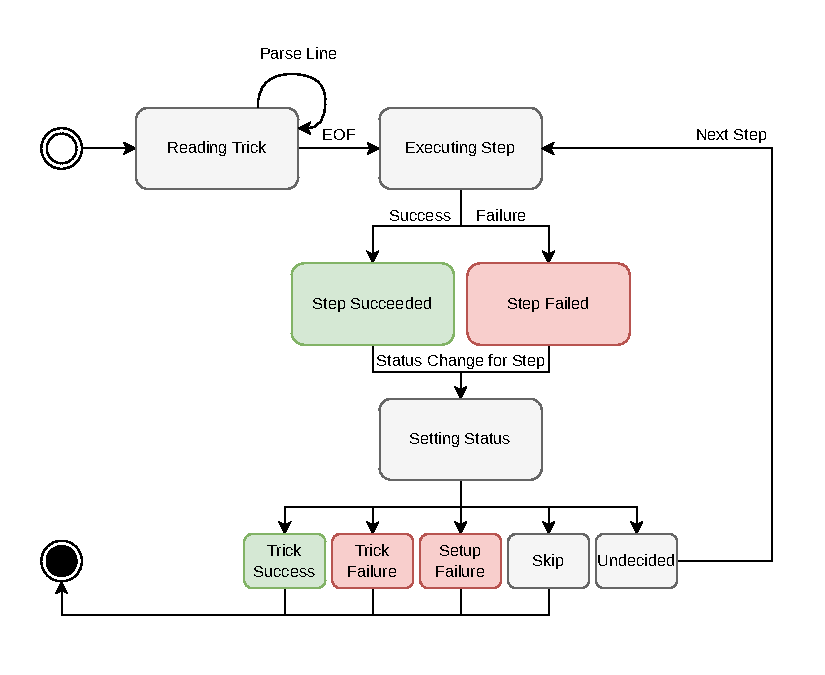
\includegraphics[width=1\linewidth]{figs/houdini-state-machine.pdf}
  \caption{A state machine diagram of Houdini running a Trick.}
\end{figure}

\section{Implementation}
\label{sec:implementation}

Tricks are divided into three separate files: a configuration file, a Python file, and a Dockerfile. Each \houdini trick begins with a configuration file (see \Cref{lst:configuration-file}), which contains the Docker container's settings and environment configuration. The configuration file defines various Docker-specific parameters that are directly fed to the Docker API to start a container with the desired settings. Once the configuration is parsed, \houdini communicates these settings to the Docker API, using Docker's docker run command to initiate the container with these parameters. This ensures that the container is launched with the exact environment specified. This automation ensures the container is started exactly as specified, and that parameters such as network mode, mounts, security options, and user privileges are all controlled from a single file. This makes it easier to test, replicate, and share container environments.


\begin{listing}[h]
  \caption{Configuration file for a default Docker out-of-the-box security settings applied when a container is launched.}
  \label{lst:configuration-file}
  \begin{minted}[frame=lines,framesep=2mm, fontsize=\scriptsize, breaklines=true]{yaml}
    name: out-of-the-box docker configuration
    dockerfile:
      - path: Dockerfile
    dependencies:
      - server: False
    docker_config: 
      - network_mode: bridge
      - read_only: False
      - security_opt: []
      - pid_mode: null
      - cpu_shares: 1024
      - volumes : []
      - mem_limit: null
      - cpuset_cpus: null
      - cpu_quota: null
      - cpu_period: null
      - cap_add: []
      - cap_drop: []
      - privileged: False
      - user: root
      - pids_limit: null
      - ipc_mode: private
    trick:
      - path: /houdini/tricks/HostMount
  \end{minted}
\end{listing}



The second component is a Python file that contains the trick implementation. This Python file is executed inside the container and is responsible for carrying out the trick scenario.


\begin{listing}[h]
  \caption{Exploit for CVE-2024-21616}
\label{lst:pythonfile}
  \begin{minted}[frame=lines,framesep=2mm, fontsize=\scriptsize, breaklines=true]{yaml}
    import os

    relative_path = '../../../../../'

    try:
        os.chdir(relative_path)
        print(f"Successfully changed directory to: {os.getcwd()}")
    except FileNotFoundError as e:
        print(f"Error: {e}")
    except PermissionError as e:
        print(f"Error: {e}")
    except Exception as e:
        print(f"Unexpected error: {e}")
  \end{minted}
\end{listing}


Finally, the Dockerfile is used to configure and set up the container's environment. It specifies how the container should be built, including copying necessary files into the container and installing required dependencies. The Dockerfile also configures the container with the settings defined in the configuration file, ensuring the container is set up correctly to run the trick.

\begin{listing}[H]
  \caption{}
\label{lst:dockerfile}
  \begin{minted}[frame=lines,framesep=2mm, fontsize=\scriptsize, breaklines=true]{yaml}
    FROM ubuntu:20.04
    RUN apt-get update -y
    WORKDIR /proc/self/fd/9
    CMD ["bash", "-c", "ls ../../../../../houdini/tricks/HostMount"]
  \end{minted}
\end{listing}

This modular design, comprising of the configuration file, Python script, and Dockerfile provides flexibility to define and test various container escapes and vulnerabilities. It also allows users to easily customize or extend existing tricks by modifying any of the three components to suit their needs.
\section{Evaluation}
\label{sec:evaluation}

To assess the effectiveness of container confinement mechanisms, we conducted a series of controlled experiments to evaluate whether common security policies successfully prevent resource starvation, unauthorized access attempts, and container escapes. Our evaluation focuses on testing various isolation features, including namespaces, cgroups, seccomp, and Linux capabilities, under different configurations and attack scenarios. These are done in the form of three case studies.










\subsection{Case Study 1: Evaluating CVE-2024-21626}

CVE-2024-21626 is a critical vulnerability affecting Docker and runc that allows malicious containers to escape their isolation and execute arbitrary commands on the host system. This poses a significant risk to enterprises relying on containerization, as attackers could gain unauthorized access to sensitive data and system resources. 

The root cause of this vulnerability lies in how runc handles cgroups for containers, which are used to manage system resources like CPU and memory. When runc creates a container, it opens a file descriptor to the host's /sys/fs/cgroup directory to configure resource limits for the container. This file descriptor is exposed inside the container via /proc/self/fd/, which lists all open file descriptors of the container's process. The vulnerability occurs when an attacker manipulates the working directory in the Dockerfile to point to a file descriptor like \texttt{/proc/self/fd/7}, which refers to the host’s /sys/fs/cgroup. By doing this, the container’s process is no longer interacting with its own filesystem but with the host’s cgroup settings, effectively breaking the container's isolation. 

To test the exploitability of CVE-2024-21626, we designed a Houdini trick that executes the following steps:
\begin{enumerate}
    \item Launch a container with various runc.
    \item Set the working directory to \texttt{/proc/self/fd/<fd>}, pointing to a controlled file descriptor.
    \item Attempt to break out of the container by leveraging the misconfigured working directory.
    \item Validate whether commands can be executed on the host system.
\end{enumerate}

The CVE for this vulnerability initially indicated that the affected runc versions were >= 1.0.0-rc93, <= 1.1.11. This suggests the vulnerability was introduced in runc version rc93 and fixed in version 1.1.12. However, empirical tests conducted by \houdini revealed a significant discrepancy with this assumption. Houdini's testing showed that earlier runc versions, such as \texttt{1.0.0-rc1}, \texttt{1.0.0-rc2}, \texttt{1.0.0-rc3}, and \texttt{1.0.0-rc4} exhibited the same vulnerability. This discovery expands upon the original CVE report's scope as the vulnerability had been present in runc versions prior to rc93.

\begin{table}[H]
    \centering
    \caption{Runc Versions Against CVE-2024-21626}
    \label{tab:cve201626}
    \resizebox{\columnwidth}{!}{%
        \begin{tabular}{l|l|c|c}
            \hline
            \textbf{Docker Version} & \textbf{Runc Version} & \textbf{Leaked FD} & \textbf{Exploit Success} \\
            \hline
            1.11.0 & runc 0.0.9 & - & \xmark \\
            1.12.0 & runc 1.0.0-rc1 & /proc/self/fd/4 & \cmark \\
            17.03.0-ce & runc 1.0.0-rc2 & /proc/self/fd/4 & \cmark \\
            17.06.1-ce & runc 1.0.0-rc3 & /proc/self/fd/5 & \cmark \\
            17.09.0-ce & runc 1.0.0-rc4 & /proc/self/fd/5 & \cmark \\
            - & runc 1.0.0-rc8 & - & \xmark \\
            - & runc 1.0.0-rc10 & - & \xmark \\
            - & runc 1.0.0-rc91 & - & \xmark \\
            20.10.17 & runc 1.1.2 & /proc/self/fd/9 & \cmark \\
            23.0.1 & runc 1.1.4 & /proc/self/fd/8 & \cmark \\
            23.0.5 & runc 1.1.5 & /proc/self/fd/8 & \cmark \\
            24.0.2 & runc 1.1.7 & /proc/self/fd/9 & \cmark \\
            24.0.5 & runc 1.1.8 & /proc/self/fd/9 & \cmark \\
            24.0.7 & runc 1.1.9 & /proc/self/fd/9 & \cmark \\
            24.0.0 & runc 1.1.11 & /proc/self/fd/9 & \cmark \\
            - & runc 1.1.12 & - & \xmark \\
            - & runc 1.1.13 & - & \xmark \\
            - & runc 1.1.14 & - & \xmark \\
            \hline
        \end{tabular}
    }
\end{table}

These findings highlight two key aspects of \houdini’s role in uncovering the true scope of the vulnerability. Firstly, it challenges misleading security assumptions. Secondly, it identifies gaps between intended and actual enforcement.

The security assumption outlined in the CVE is that the vulnerability exists only in runc versions >= 1.0.0-rc93, <= 1.1.11, suggesting that earlier versions are safe. This creates a false sense of security, leading users and system administrators to believe there is no urgency to patch or retire older versions. Rather than accepting the CVE’s claims, \houdini takes a more rigorous approach by testing the actual behavior of the continaer to determine whether the vulnerability is present in those earlier versions. In doing so, \houdini follows a fundamental security principle: security must be validated through testing, not simply assumed or trusted. 

While security policies and CVEs often describe what should be true, such as which versions are affected or which behaviors are restricted, what actually happens at runtime can tell a different story. Houdini helps expose these gaps between what is stated in documentation and how the system behaves in practice by testing the system in real-world scenarios. For example, while the CVE marked runc version 1.0.0-rc93 as the point where the vulnerability was introduced, Houdini’s testing revealed that the issue existed in earlier versions as well, showing that isolation was already broken. This mismatch between what is expected and what is actually happening can lead to serious problems. Organizations may rely on official documentation and assume their systems are safe, overlooking vulnerabilities that fall outside the scope of the CVE. As a result, they might miss critical risks, leaving systems unpatched and vulnerable to exploitation. By testing how the container behaves under specific configurations, Houdini provides a more accurate picture of the system’s security, which helps to uncover vulnerabilities that might otherwise be overlooked.



\captionof{listing}{Configuration file for Case Study I}
\label{lst:configuration-file}
\begin{minted}[frame=lines,framesep=2mm, fontsize=\scriptsize, breaklines=true]{yaml}
name: host_mount
dockerfile:
  - path: Dockerfile
dependencies:
  - server: False
  - security_opt: null
docker_config: 
  - network_mode: bridge
  - read_only: False
  - security_opt: []
  - pid_mode: null
  - cpu_shares: 1024
  - volumes : []
  - mem_limit: null
  - cpuset_cpus: null
  - cpu_quota: null
  - cpu_period: null
  - cap_add: []
  - cap_drop: []
  - privileged: False
  - user: root
  - pids_limit: null
  - ipc_mode: null
trick:
  - path: /houdini/tricks/HostMount
\end{minted}

\vspace{1em}

\captionof{listing}{Trick Implementation for Case Study I}
\label{lst:pythonfile}
\begin{minted}[frame=lines,framesep=2mm, fontsize=\scriptsize, breaklines=true]{bash}
#!/bin/bash
relative_path='../../../../../'
target_file='houdini/tricks/HostMount/61240abcc5412ab'

if cd "$relative_path" 2>/dev/null; then
    echo "Successfully changed directory to: $(pwd)"

    if [ -f "$target_file" ]; then
        echo "File found: $target_file"
    else
        echo "File not found: $target_file"
    fi
else
    err_code=$?
    case $err_code in
        1)
            echo "Error: Permission denied"
            ;;
        2)
            echo "Error: No such file or directory"
            ;;
        *)
            echo "Unexpected error (exit code $err_code)"
            ;;
    esac
fi

echo "Docker version:"
docker --version || echo "Docker not found"

echo "runc version:"
runc --version || echo "runc not found"

\end{minted}

\vspace{1em}

\captionof{listing}{Dockerfile for Case Study I}
\label{lst:dockerfile}
\begin{minted}[frame=lines,framesep=2mm, fontsize=\scriptsize, breaklines=true]{dockerfile}
FROM ubuntu:16.04
WORKDIR /proc/self/fd/4
COPY host_mount.sh /host_mount.sh
RUN chmod +x /host_mount.sh
CMD ["/host_mount.sh"]
\end{minted}









\subsection{Case Study 2 - Evaluating Host Process Manipulation via PID Namespace Escape}

In this evaluation, we investigate whether a Docker container running with \texttt{--pid=host} can interact with and manipulate host processes. The PID namespace is responsible for process isolation, ensuring that containerized processes remain separate from host processes. However, when \texttt{--pid=host} is enabled, the container shares the host's PID namespace, making all host processes visible inside the container. We assess the security implications of this setting by evaluating the following:

\begin{itemize}
    \item Whether a container with \texttt{--pid=host} can list host processes.
    \item Whether the container can send signals \texttt{SIGKILL}, \texttt{SIG\-TERM} to host processes.
    \item Whether enabling \texttt{CAP\-\_SYS\_ADMIN} allows process tracing of host processes.
    \item Whether a container can read host process memory via \texttt{/proc/\$PID/mem}.
\end{itemize}

\begin{table}[h!]
\caption{Testing Environment}
\centering
\scriptsize % Reduces font size more
\begin{tabular}{|l|l|} 
\hline
\textbf{Component} & \textbf{Specification} \\
\hline
Host Machine & 20 Core CPU, 16GB RAM, Ubuntu 24.04 \\
\hline
Virtual Machine & QEMU, 4 Core CPU, 12GB RAM, No Distribution \\
\hline
Docker Version & 27.0.3 \\
\hline
Kernel Version & 5.4 \\
\hline
Container Runtime & \texttt{runc} 1.1.11 \\
\hline
\end{tabular}
\end{table}

The container was started with various security configurations:

\begin{itemize}
    \item Default Docker container configuration (separate PID namespace)
    \item Docker container with \texttt{--pid=host}
    \item Docker container with \texttt{--pid=host} and additional capabilities \texttt{CAP\_KILL}, \texttt{CAP\_SYS\_PTRACE}
    \item Docker container with \texttt{--pid=host} and additional capabilities \texttt{CAP\_SYS\_PTRACE}
    \item Privileged Docker container with \texttt{--pid=host}
\end{itemize}

For each security configuration, different methods were tested to determine whether a process inside the container could interact and/or manipulate host processes.

The evaluation began by assessing whether a container with \texttt{--pid=host} could list host processes using \texttt{ps aux}. As expected, the container displayed all host processes, confirming that sharing the host PID namespace fully exposes the host process table. 

Following this, we tested whether the container could send termination signals (\texttt{SIGKILL}, \texttt{SIGTERM}) to host processes using \texttt{kill -9 <PID>}. Without the \texttt{CAP\_KILL} capability, the operation was not permitted. However, enabling \texttt{CAP\_KILL}  process termination within the namespace's limits, and granting \texttt{--privileged} access enabled the container to kill any host process. 

Next, we investigated whether the container could attach a debugger to host processes via \texttt{strace -p <PID>}. Without \texttt{CAP\_SYS\_PTRACE}, the operation was denied, but enabling this capability  successful attachment to a host process, raising concerns about potential leakage of sensitive data through system call tracing. 

We then examined whether the container could read host process memory by attempting to access \texttt{/proc/<host\_pid>/mem}. With Docker’s default restrictions, the operation was denied, but when running the container with \texttt{--privileged}, the process memory could be read using \texttt{cat /proc/<host\_pid>/mem}. 

Finally, we tested cross-container process manipulation by launching two containers with \texttt{--pid=host}. A process running in Container A (e.g., \texttt{sleep 1000}) was visible to Container B, which was able to list and terminate it, proving that containers sharing the host PID namespace are not isolated from each other and can manipulate each other's processes.

The result was that the process inside Container A was visible to Container B, and it could be terminated using \texttt{kill -9 <PID>}, proving that containers with \texttt{--pid=host} share the same namespace and are not isolated from each other.

The effectiveness of different configurations in preventing host and cross-container process manipulation is also illutrated in Table~\ref{tab:pid-namespace-security}.

This case study highlights a core strength of \houdini, which is its ability to systematically explore and identify the least privilege for a given operation. By allowing users to declaratively modify container configurations, \houdini makes it easy to test a wide range of privilege combinations in a repeatable and automated way. Instead of relying on trial-and-error or defaulting to the overly permissive \texttt{--privileged} mode, users can incrementally grant permissions and observe the effect of each change. This enables security practitioners, developers, and researchers to precisely determine the minimum set of permissions required for a given trick to succeed. As a result, \houdini not only serves as a testing framework for container escapes and misconfigurations, but also as a practical tool for privilege minimization and hardening container deployments.

This case study also highlights a scenario where the security policies administrators intend to implement are not properly enforced when the container is running. For example, an administrator may want to use the host's process namespace for tracing host processes but restrict the container from manipulating those processes. To achieve this, the administrator configures the container with \texttt{--pid=host}. \houdini validates this configuration by performing controlled tests to ensure the container can only trace processes and cannot send signals, attach debuggers, or read process memory. If \houdini detects that the container can perform any of these unauthorized actions, it reveals a gap between the intended policy and its actual enforcement. Houdini’s tests provide actionable insights that help administrators adjust configurations to enforce proper isolation while allowing the container to trace processes.

\FloatBarrier
\begin{table*}[h]  
    \centering
    \footnotesize  
    \setlength{\tabcolsep}{4pt}  
    \renewcommand{\arraystretch}{1.1}  
    \caption{Ability for container configurations to interact with host processes}
    \label{tab:pid-namespace-security}  
    \begin{adjustbox}{max width=\textwidth}  
    \begin{tabular}{|l|c|c|c|c|c|c|c|}
        \hline
        \textbf{\texttt{Security Configuration}} & \textbf{\texttt{--pid=host}} & \textbf{\texttt{CAP\_KILL}} & \textbf{\texttt{CAP\_SYS\_PTRACE}} & \textbf{\texttt{--privileged}} & \textbf{\texttt{--pid=host} + \texttt{--user=non-root}} & \textbf{\texttt{--pid=host} + \texttt{apparmor=docker-default}}  \\ \hline
        \textbf{\texttt{--pid=host}} & $\diamondsuit$ & $\diamondsuit$ $\triangle$ & $\diamondsuit$ $\star$ & $\diamondsuit$ $\triangle$ $\star$ $\square$ & $\diamondsuit$ & $\diamondsuit$ \\ \hline
        \textbf{\texttt{CAP\_KILL}} & $\diamondsuit$ $\triangle$ & & & & $\diamondsuit$ & $\diamondsuit$  \\ \hline
        \textbf{\texttt{CAP\_SYS\_PTRACE}} & $\diamondsuit$ $\star$ & & & $\diamondsuit$ & $\diamondsuit$ & $\diamondsuit$ \\ \hline
        \textbf{\texttt{--privileged}} & $\diamondsuit$ $\triangle$ $\star$ $\square$ & & & & $\diamondsuit$ $\triangle$ $\star$ $\square$ \\ \hline
        \textbf{\texttt{--pid=host} + \texttt{--user=non-root}} & $\diamondsuit$ & $\diamondsuit$  & $\diamondsuit$ & $\diamondsuit$ $\square$ & $\diamondsuit$ $\square$ \\ \hline
        \textbf{\texttt{--pid=host} + \texttt{apparmor=docker-default}} & $\diamondsuit$ & $\diamondsuit$ $\triangle$ & $\diamondsuit$ & $\diamondsuit$ $\triangle$ $\star$ $\square$ \\ \hline 

    \end{tabular}  
    \end{adjustbox}  
    \vspace{0.5em} \\
    \noindent\textbf{Legend} \\
    $\diamondsuit$ List Host Processes \quad
    $\triangle$ Send Signals \quad
    $\star$ Attach Debugger \quad
    $\square$ Read Memory
\end{table*}





\captionof{listing}{Configuration file for Case Study I}
\label{lst:configuration-file}
\begin{minted}[frame=lines,framesep=2mm, fontsize=\scriptsize, breaklines=true]{yaml}
name: host_network_namespace
dockerfile:
  - path: Dockerfile
dependencies:
  - server: True
docker_config: 
  - network_mode: bridge
  - read_only: False
  - security_opt: []
  - pid_mode: null
  - cpu_shares: null
  - volumes: null
  - mem_limit: null
  - cpuset_cpus: null
  - cpu_quota: null
  - cpu_period: null
  - cap_add: []
  - cap_drop: []
  - privileged: False
  - user: myuser
  - pids_limit: null
  - ipc_mode: null
trick:
  - path: /houdini/tricks/ProcessNamespace
\end{minted}

\vspace{1em}

\captionof{listing}{Trick Implementation for Case Study I}
\label{lst:pythonfile}
\begin{minted}[frame=lines,framesep=2mm, fontsize=\scriptsize, breaklines=true]{bash}
#!/bin/bash

TARGET_CMD="python3 /houdini/server.py"
PID=""

find_target_process() {
    echo "[1] Searching for process: $TARGET_CMD"
    PID=$(ps aux | grep '[p]ython3 /houdini/server.py' | awk '{print $2}' | head -n 1)
    if [[ -n "$PID" ]]; then
        echo "Found: PID=$PID"
        return 0
    else
        echo "Target process not found."
        return 1
    fi
}

send_signal() {
    echo "[2] Sending SIGCONT to PID $PID"
    if kill -CONT "$PID" 2>/dev/null; then
        echo "Signal sent successfully"
    else
        echo "Failed to send signal"
    fi
}

attach_debugger() {
    echo "[3] Attaching debugger with ptrace to PID $PID"
    if strace -p "$PID" -e trace=none -o /dev/null -t -qq &>/dev/null & sleep 1; then
        echo "Able to attach (via strace)"
        pkill -P $$ strace 2>/dev/null
    else
        echo "Failed to attach debugger"
    fi
}

read_memory() {
    echo "[4] Trying to read memory from /proc/$PID/mem"
    if dd if="/proc/$PID/mem" bs=1 count=4 skip=0 2>/dev/null | hexdump; then
        echo "Read memory succeeded"
    else
        echo "Failed to read memory"
    fi
}

main() {
    find_target_process || exit 1
    echo
    send_signal
    echo
    attach_debugger
    echo
    read_memory
}

main
\end{minted}

\vspace{1em}

\captionof{listing}{Dockerfile for Case Study I}
\label{lst:dockerfile}
\begin{minted}[frame=lines,framesep=2mm, fontsize=\scriptsize, breaklines=true]{dockerfile}
FROM ubuntu:20.04

RUN apt-get update && \
    apt-get install -y python3

WORKDIR /
RUN useradd -m myuser
COPY process_namespace.sh /process_namespace.sh
RUN chmod +x /process_namespace.sh
USER myuser
CMD ["/bin/bash", "/process_namespace.sh"]
\end{minted}
























\subsection{Case Study 2 - Evaluating Docker Privileged Port Forwarding Restrictions}

In this case study, we evaluate Docker’s network isolation mechanisms to determine how well they enforce privileged port binding restrictions. Starting with Docker version 20.03, a significant change was introduced to Docker. They redefined unprivileged ports to start at 0 instead of 1024, effectively removing the need for root to bind to privileged ports. Table ~\ref{tab:port-binding-pre-20.03} presents the results.

\begin{table*}[h]
    \centering
    \caption{Ability for Container to bind to privileged ports}
    \label{tab:port-binding-pre-20.03}
    \scriptsize
    \begin{tabular}{|p{2.5cm}|c|c|c|c|c|}
        \hline
        \texttt{Docker Version} & \texttt{NET\_BIND\_SERVICE + root} & \texttt{NET\_BIND\_SERVICE + root-less} & \texttt{root} & \texttt{root-less} & \texttt{Default Container (Bridge Mode)} \\ \hline
        19.03.9                & \cmark                         & \xmark                               & \xmark      & \xmark           & \xmark                                      \\ \hline
        19.03.0                & \cmark                         & \xmark                               & \xmark      & \xmark           & \xmark                                      \\ \hline
        20.10.0                & \cmark                         & \xmark                              & \xmark      & \xmark           & \xmark                                      \\ \hline
        20.10.3                & \cmark                         & \xmark                              & \xmark      & \xmark           & \xmark                                      \\ \hline
        23.0.0                 & \cmark                         & \cmark                              & \cmark      & \xmark           & \xmark                                      \\ \hline
        25.0.0                 & \cmark                         & \cmark                              & \cmark      & \xmark           & \xmark                                      \\ \hline
        27.0.1                 & \cmark                         & \cmark                              & \cmark      & \xmark           & \xmark                                      \\ \hline
    \end{tabular}
\end{table*}

This case study highlights how discrepancies between Docker versions in handling privileged port binding can create gaps between administrators' intended confinement policies and actual enforcement. A change in Docker's handling of binding to privileged ports, such as the removal of the NET\_BIND\_SERVICE requirement starting from Docker 20.03, may allow containers to bypass restrictions even when policies are set to prevent it. 

For example, administrators might configure a container to be restricted from binding to privileged ports, but if Docker is running a version where the NET\_BIND\_SERVICE capability is no longer required for root containers (like in Docker 20.03 and beyond), the container could still bind to these ports despite the policy specifying otherwise. This creates a mismatch between the intended policy (restricting privileged port binding) and the actual enforcement (where containers can still bind to those ports in certain Docker versions).

Houdini helps identify these gaps by systematically testing container configurations across different Docker versions. By simulating different Docker versions and security policies, Houdini verifies whether containers are correctly enforcing the intended restrictions on privileged port binding. For instance, Houdini could test whether containers configured to prevent binding to privileged ports are still able to bind to those ports in Docker versions 20.03 or later, where the security model has changed. If a container running with Docker 20.03 or newer can bind to privileged ports despite the configuration specifying otherwise, Houdini will detect this discrepancy and highlight the gap between the intended policy and actual enforcement.

This set of experiments evaluates how Docker’s privilege model for binding to privileged ports (i.e., ports below 1024) has evolved across versions. Traditionally, binding to privileged ports required root access or the NET\_BIND\_SERVICE capability. However, newer versions of Docker introduced support for binding to these ports even in rootless containers, provided the necessary capability is explicitly granted.

By testing various combinations of user privileges (root vs. rootless) and capability settings across multiple Docker versions, this case study reveals which configurations are sufficient and which are excessive for achieving the goal of binding to a low-numbered port. It demonstrates that in modern Docker versions (23.0.0+), it is no longer necessary to run as root or grant all privileges to perform this operation. Instead, a least-privileged approach using a rootless container with NET\_BIND\_SERVICE is sufficient.

This case study shows that \houdini can empower Docker users to avoid unnecessary elevation of privileges, particularly avoiding full root access or the use of the --privileged flag, both of which expose containers to a broader attack surface. Houdini enables this kind of analysis by systematically testing Docker configurations and identifying the minimum set of privileges required for a given operation, helping developers and administrators adopt safer, more secure defaults.





\captionof{listing}{Configuration file for Case Study I}
\label{lst:configuration-file}
\begin{minted}[frame=lines,framesep=2mm, fontsize=\scriptsize, breaklines=true]{yaml}
name: cpu_shares
dockerfile:
  - path: Dockerfile
dependencies:
  - server: False
docker_config: 
  - network_mode: bridge
  - read_only: True
  - security_opt: []
  - pid_mode: null
  - cpu_shares: 512
  - volumes : []
  - mem_limit: null
  - cpuset_cpus: null
  - cpu_quota: null
  - cpu_period: null
  - cap_add: ["NET_BIND_SERVICE"]
  - cap_drop: []
  - privileged: False
  - user: root
  - pids_limit: null
  - ipc_mode: null
trick:
  - path: /houdini/tricks/PrivilegedPorts
\end{minted}

\vspace{1em}

\captionof{listing}{Trick Implementation for Case Study I}
\label{lst:pythonfile}
\begin{minted}[frame=lines,framesep=2mm, fontsize=\scriptsize, breaklines=true]{bash}
import http.server
import socketserver

PORT = 23

Handler = http.server.SimpleHTTPRequestHandler

try:
    # Try to bind to the port without serving
    with socketserver.TCPServer(("", PORT), Handler) as httpd:
        print(f"Successfully bound to port {PORT}")
except PermissionError as e:
    print(f"Failed to bind to port {PORT}: {e}")

\end{minted}

\vspace{1em}

\captionof{listing}{Dockerfile for Case Study I}
\label{lst:dockerfile}
\begin{minted}[frame=lines,framesep=2mm, fontsize=\scriptsize, breaklines=true]{dockerfile}
FROM python:3.9-slim
RUN groupadd -r myuser && useradd -r -g myuser myuser
WORKDIR /
COPY privileged_ports.py /privileged_ports.py
RUN chown myuser:myuser privileged_ports.py 
USER root
CMD ["python", "privileged_ports.py"]
\end{minted}
\section{Related Work}%
\label{sec:related}

At the time of this writing, to our knowledge, Houdini is the first comprehensive approach for evaluating and comparing \textit{container confinement mechanisms}. Much of the container security literature to date has focused on either vulnerability scanning of container images, building offensive/attack tools for container escapes, or proposing best practices for securing container runtimes. While these papers, tools, and documents do not directly share our research objectives, they still broadly fit into the container security landscape. Additionally, research on VM escapes and sandbox escapes has provided valuable insights into isolation vulnerabilities, many of which relate to container security. Techniques used to break out of hypervisors and sandboxed environments often share similarities with container escape methods, which the importance of strong confinement mechanisms. The remainder of this section does not aim to exhaustively enumerate all container security tools and systems, but rather to highlight the various salient methods, including prior research on times the confinement of VMs and sandboxes have been escaped as it is  related to work.

\noindent\textbf{Vulnerability Scanners.} Many free, open, and closed-source tools exist for identifying the presence of known vulnerabilities in container images. Shu \etal~\cite{shu2017study} developed a vulnerability scanning tool to scan Docker Hub container images at scale. They found that on average, official and community images have concerning amounts of vulnerabilities (180+), and that these vulnerabilities remain unpatched for hundreds of days. Their study utilized the Docker Image Vulnerability Analysis (DIVA) framework, which automates the discovery, download, and analysis of over 300,000 Docker images. The findings revealed that more than 80\% of both official and community images contained at least one high-severity vulnerability, and many images were not updated for extended periods. Moreover, vulnerabilities were often inherited from parent images to child images, further increasing security risks.

\noindent\textbf{Best Practices.} Users in search of (often high-level) advice on how to improve the security of their container deployments can consult one of many best practices guides available online. One such guide is the Center for Interent Security (CIS) Docker Benchmark \cite{CIS}. In our experience, guides tend to offer generic advice (e.g., ``\textit{Only allow read access to the root filesystem}''. This is problematic because it oversimplifies container security. Generic advice like "Only allow read access to the root filesystem" may seem straightforward, but it doesn't account for the specific context or unique configuration of an individual deployment. Such one-size-fits-all recommendations can lead users to believe that simply following these broad guidelines is enough to secure their systems, potentially leaving critical vulnerabilities unaddressed. In reality, effective container security requires a nuanced, tailored approach that considers the particular needs and threat models of each environment. Houdini fills the gap between generic advice and practical security by enabling you to objectively evaluate the effectiveness of your container confinement measures.

\noindent\textbf{Offensive Tools.} The offensive security community has developed a range of specialized tools aimed at identifying and exploiting vulnerabilities within containerized environments. Containers, while providing strong isolation, are not immune to attacks, and these tools focus on testing the robustness of container defenses. CDK\footnote{\url{https://github.com/cdk-team/CDK}} and DEEPCE\footnote{\url{https://github.com/stealthcopter/deepce}} are two widely used, open-source container penetration testing toolkits that leverage a collection of known exploits to gain persistence, escape the container, and gather sensitive information about the container environment. These tools aim to bypass isolation mechanisms like namespaces, cgroups, and SELinux, often using a variety of aggressive techniques to identify weaknesses in container security. CDK specifically uses any available method to circumvent security measures, providing a broad toolkit to test the limits of a container’s defense. Meanwhile, DEEPCE, developed by stealthcopter, focuses on privilege escalation and container enumeration, attempting to exploit specific weaknesses to achieve container escapes, thereby compromising the host system. In contrast, Houdini takes a more systematic and structured approach to container security testing. Rather than focusing solely on exploiting vulnerabilities, Houdini allows for the direct comparison of defensive techniques by clearly defining the testing environment, outlining the exploit steps, and documenting the expected outputs.

\noindent\textbf{Virtual Machine Escapes} VM escapes occur when an attacker successfully breaks out of a virtualized confined environment, gaining unauthorized access to the host system. Given that hypervisors manage multiple VMs on shared hardware, such escapes can lead to host compromise, cross-VM attacks, and lateral movement within cloud environments. One of the most notable VM escape vulnerabilities is VENOM (CVE-2015-3456) \cite{abdoul2018novel}, which exploited a flaw in the virtual floppy disk controller (FDC) implementation in QEMU, affecting platforms like Xen, KVM, and VirtualBox. Other significant VM escape vulnerabilities include Cloudburst (2009), which exploited VMware's virtual graphics driver; CVE-2018-6981 and CVE-2018-6982, which targeted VMware ESXi, Workstation, and Fusion \cite{vmware2018escape}; and multiple VirtualBox vulnerabilities (2017) enabling guest-to-host code execution \cite{virtualbox2017bugs}. Additionally, side-channel attacks like MDS/ZombieLoad (2019) demonstrated how speculative execution flaws could be leveraged across VMs \cite{mds2019attack}. More recent research has uncovered weaknesses in encrypted virtualization, such as the SEVered attack (2018), which extracted plaintext memory from AMD SEV-protected VMs \cite{severed2018}, and the Heckler attack (2024), which manipulated non-timer interrupts to compromise confidential VMs in AMD SEV-SNP and Intel TDX \cite{heckler2024}.

\noindent\textbf{Sandbox Escapes} Sandboxing is a critical security mechanism for restricting the execution of untrusted code, commonly used in browsers, mobile apps, and security tools. A sandbox escape occurs when an attacker bypasses these restrictions, executing arbitrary code with higher privileges and potentially leading to full system compromise. Modern web browsers heavily rely on sandboxing to isolate JavaScript execution from the underlying OS. However, several high-profile vulnerabilities have enabled sandbox escapes. For example, CVE-2019-5786 \cite{chromezeroday}, a use-after-free vulnerability in the FileReader API of Google Chrome, allowed attackers to escape Chrome's sandbox and execute code on the host. Other notable sandbox escape vulnerabilities include CVE-2022-26706, which exploited a flaw in macOS's App Sandbox to execute code outside of restricted permissions \cite{macossandboxescape}; CVE-2023-36719, a stack corruption vulnerability in Windows OS that enabled escape from the Chromium sandbox \cite{chromiumsandboxescape}; and CVE-2024-4040, which was actively exploited to break out of CrushFTP’s Virtual File System (VFS) \cite{crushftpsandboxescape}. Additionally, vulnerabilities in Judge0, an online code execution system, exposed systems to full takeover by allowing attackers to escape its sandbox \cite{judge0sandboxescape}. Research has also uncovered critical flaws in vm2, a JavaScript sandbox library, which could be exploited to bypass its security restrictions and gain remote code execution \cite{vm2sandboxescape}.
\section{Discussion}
\label{sec:discussion}
Houdini’s design not only addresses critical security challenges in container confinement but also lends itself well to continuous security testing in modern software development environments. Because it is both safe and modular, \houdini can be seamlessly integrated into automated systems, such as CI/CD pipelines, to provide ongoing validation of container security.

Regression testing is a widely adopted practice in software engineering to ensure that updates or changes to code do not introduce unintended failures or security regressions. In the context of container security, integrating \houdini into CI/CD pipelines enables organizations to automatically trigger a comprehensive suite of confinement tests whenever any part of the container stack changes—such as kernel upgrades, Docker releases, or policy updates. This continuous validation ensures that every new deployment or system update is accompanied by an up-to-date security assessment. By systematically rerunning empirical security tests across different software versions and configurations, \houdini helps detect configuration drift and regression in security guarantees that might otherwise go unnoticed, maintaining the effectiveness of container isolation mechanisms as platforms evolve.
\section{Conclusion}
\label{sec:conclusion}

In this paper, we presented Houdini, a security benchmarking framework designed to evaluate the effectiveness of container confinement mechanisms. As container-based workloads continue to dominate cloud infrastructures, ensuring that containers are properly isolated is paramount for maintaining security. Houdini offers a systematic and empirical approach to test and assess various container security configurations, highlighting potential misconfigurations that may compromise container isolation. Our evaluation demonstrated the ability of Houdini to detect critical misconfigurations, including those leading to privilege escalation. By providing a reliable and reproducible method for testing container confinement, Houdini helps bridge the gap between theoretical security assumptions and practical real-world behavior.

As container technologies evolve, it is essential to continuously assess and improve their security mechanisms. Houdini's modular design ensures that it remains adaptable to new security challenges and configurations, allowing for ongoing validation and refinement of container security practices. By offering an open framework for container confinement benchmarking, Houdini aims to support the development of more secure container technologies, ultimately contributing to a safer cloud infrastructure for the future.


\bibliographystyle{unsrt}
\bibliography{refs}
\end{document}
